\documentclass[a4paper,itemph]{oblivoir}
\setmainhangulfont{NANUMMYEONGJO.TTF}[BoldFont={NANUMMYEONGJOBOLD.TTF}]
\usepackage[english]{babel}
\usepackage[utf8x]{inputenc}
\usepackage[T1]{fontenc}
\usepackage{indentfirst}
%% Sets page size and margins
\usepackage[a4paper,top=3cm,bottom=2cm,left=3cm,right=3cm,marginparwidth=1.75cm]{geometry}

%% Useful packages
\usepackage{amsfonts}
\usepackage{amsmath}
\usepackage{graphicx}
\usepackage{subcaption}
\usepackage{amssymb}
\usepackage{amsthm}
\newtheorem{thm}{Theorem}[subsection]
\newtheorem{lem}{Lemma}[subsection]
\newtheorem{cor}{Corollary}[subsection]
\newcommand{\overbar}[1]{\mkern 1.5mu\overline{\mkern-1.5mu#1\mkern-1.5mu}\mkern 1.5mu}
\theoremstyle{definition}
\newtheorem{defn}{Definition}[subsection]
\newtheorem{rem}{Remark}[subsection]

\title{내용물 양을 알려주는 용기}
\author{권대원, 손태준, 이승준, 이준협, 허상혁\thanks{{서울대학교 전기정보공학부, 설승기 교수님 반 프로젝트 14조. \newline 학번: 순서대로 2018-14870, 2018-16692, 2018-16944, 2018-12602, 2016-19417}}}
\begin{document}
\maketitle

\begin{abstract}
이 보고서에서는 용기에서 액체를 따라내기 전 뿐만 아니라, 액체를 따르는 도중에도 용기 속에 남아있는 액체의 양을 실시간으로 시각화해줄 수 있는 회로를 제안한다. 이 회로는 값싼 op amp와 comparator, 그리고 저항만을 이용해서 구성되었기에 가격 경쟁력을 가지고 있다. 또한, 소자를 추가해서 액체의 양을 더 세밀하게 표현하려 할 때에도 threshold를 조절해서 사용할 수 있는 확장성이 좋은 회로이다. 뿐만 아니라, 액체의 종류에 관련 없이 전기 분해의 영향을 최소화시키려 구성한 회로이다. 실제로 구현한 회로는 부피가 크고 1/4 간격으로밖에 양을 표시해주지 못하지만, 더 좋은 기술로 소형화 작업을 거치고 소자를 추가하면 실제 용기에도 쓸 수 있을 정도의 가치를 가지고 있다고 예상한다.
\end{abstract}

\section{서론}
\subsection{동기}
용기를 기울여서 액체를 따라내야 하는 상황, 예를 들어 술자리에서 친구에게 술을 따라주거나, 산행 중에 다른 친구의 빈 물통에 물을 따라줘야 하는 상황을 고려해보자. 이 때 항상 문제가 되는 것은, 따르는 중에는 수면이 기울어져 있기 때문에 따라낸 물의 양을 가늠하기 어렵다는 점이다. 이 문제를 해결하기 위해 용기가 기울어져서 액체를 따라낼 때 용기에 남아있는 액체의 양을 알려주는 회로가 있는지를 검색해보게 되었다. 이미 있는 회로들의 경우, 주로 물탱크 등 내부가 보이지 않으며 물이 많이 들어있어 잔량을 확인하기 힘든 상황에서 측정이 이루어지는 경우가 많았으며 \cite{1}, 위와 같은 문제 상황을 직접적으로 다루는 회로는 찾기 어려웠다. 이에 이 문제에 특화된 제품을 제작해볼 필요성을 느껴 프로젝트를 시작하게 되었다. 

\subsection{제품 요구사양}
실제로 사용할 수 있는 제품을 만들기 위해 최소한의 요구사양을 다음과 같이 설정했다:
\begin{itemize}
    \item 적어도 1/4 간격으로 물의 잔량을 표시해준다(반을 따라낸 후, 그 반을 또 따라낼 수 있도록).
    \item 따르지 않고 있을 때와 따르고 있을 때의 모든 경우에 작동한다 (불투명한 용기의 경우를 위해).
    \item 액체이기 때문에 발생하는 전기분해 등의 현상을 최소로 한다.
\end{itemize}
액체를 다루는 프로젝트이기 때문에 상황에 따라 입력단에 연결되는 저항이 수시로 바뀐다는 문제가 있다. 이를 고려해서 회로를 짜는 것이 이 프로젝트의 관건이었다.
\section{본론}
\subsection{회로 설계}
물의 양을 전기적으로 처리하기 위해서는 물의 양에 비례하는 값을 전압으로 바꾸어줄 필요가 있다. 이 프로젝트에서는 컵 속의 특정 지점들에 전선들을 노출시켜 놓고, 물에 접촉한 전선의 개수를 물의 양과 연관시키기로 하였다. 이후 물에 접촉한 전선의 개수에 따라 변화하는 전압을 만들어낼 수 있으면, 물의 잔량에 비례하는 출력을 만들어낸 것이 되기 때문이다.
\subsubsection{아두이노}
\begin{figure}[h]
\centering
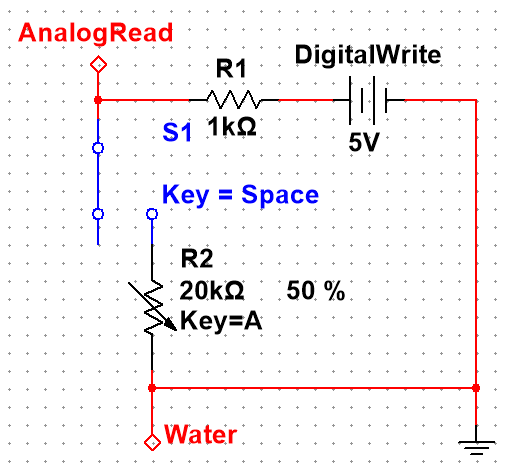
\includegraphics[width=0.3\textwidth]{arduino.PNG}
\caption{아두이노를 이용한 회로}
\end{figure}
프로젝트의 실현 가능성을 검증하기 위해 먼저 간단한 아두이노 회로를 통해 제품을 제작해보았다. 아두이노 회로는 Figure 1에서와 같이 나타낼 수 있다. analogRead가 가능한 단자, 예를 들어 A0 단자에 연결된 전선이 물에 연결되지 않았을 때에는 5[V]가 인가되고, 물에 연결되었을 때에는 물에 연결된 GND에 의해 5[V]가 divide된 더 작은 전압이 인가되게 된다. 이 때 프로그램을 사용해서 일정 threshold보다 낮은 입력이 들어오면 그 analog 단자에 해당하는 LED가 켜지도록, 즉 그 analog 단자에 연결된 전선이 물에 접촉하면 LED가 켜지도록 했다. 여기에서 20[k$\Omega$]의 가변저항은 GND와 전선 사이의 변화하는 저항을 나타내고, analog 단자의 입력 저항이 수 G$\Omega$ 단위이기 때문에 입력 쪽으로 전류가 들어가지 않는다고 가정했을 때 얻을 수 있는 결과이다.

위와 같은 회로를 이용하여 실험을 했을 때, 5[V]가 1023으로 환산되면 threshold가 980대로, 노이즈가 들어갔을 경우 아날로그 소자로 측정하기 힘든 정도의 미세한 차이를 보임을 알 수 있었다. 또한, 위 회로에서는 물에 전압이  인가되기 때문에, 전기분해가 일어남을 확인할 수 있었다. 즉, 요구 사양을 완전히 만족시키지 못했다.

\subsubsection{아날로그 회로}

\begin{figure}[!htb]
\minipage{0.32\textwidth}
  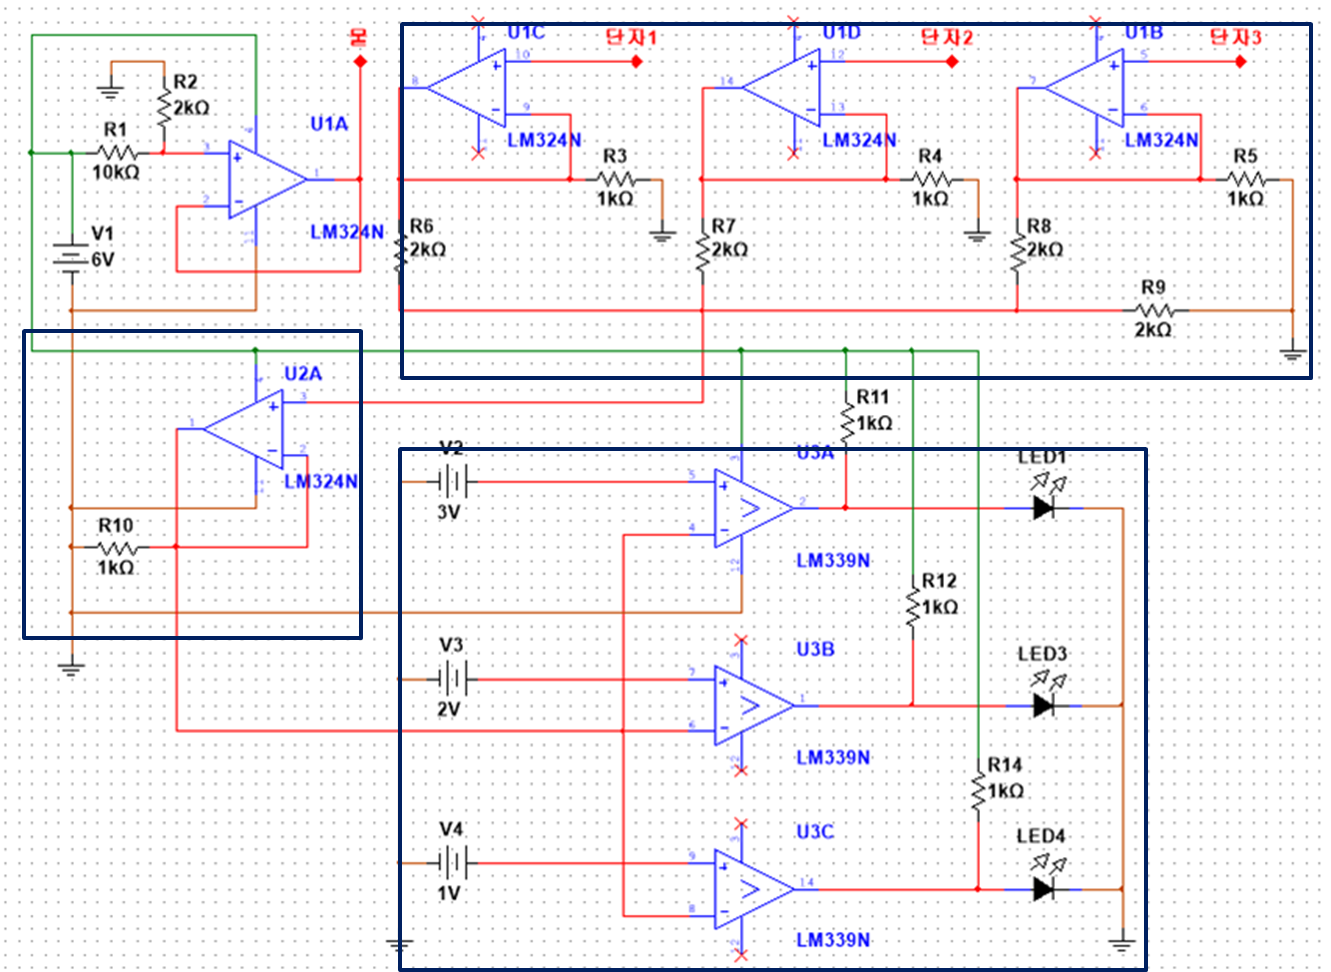
\includegraphics[width=\linewidth]{1st.png}
  \caption{중간 발표 때의 회로}\label{fig:awesome_image1}
\endminipage\hfill
\minipage{0.32\textwidth}
  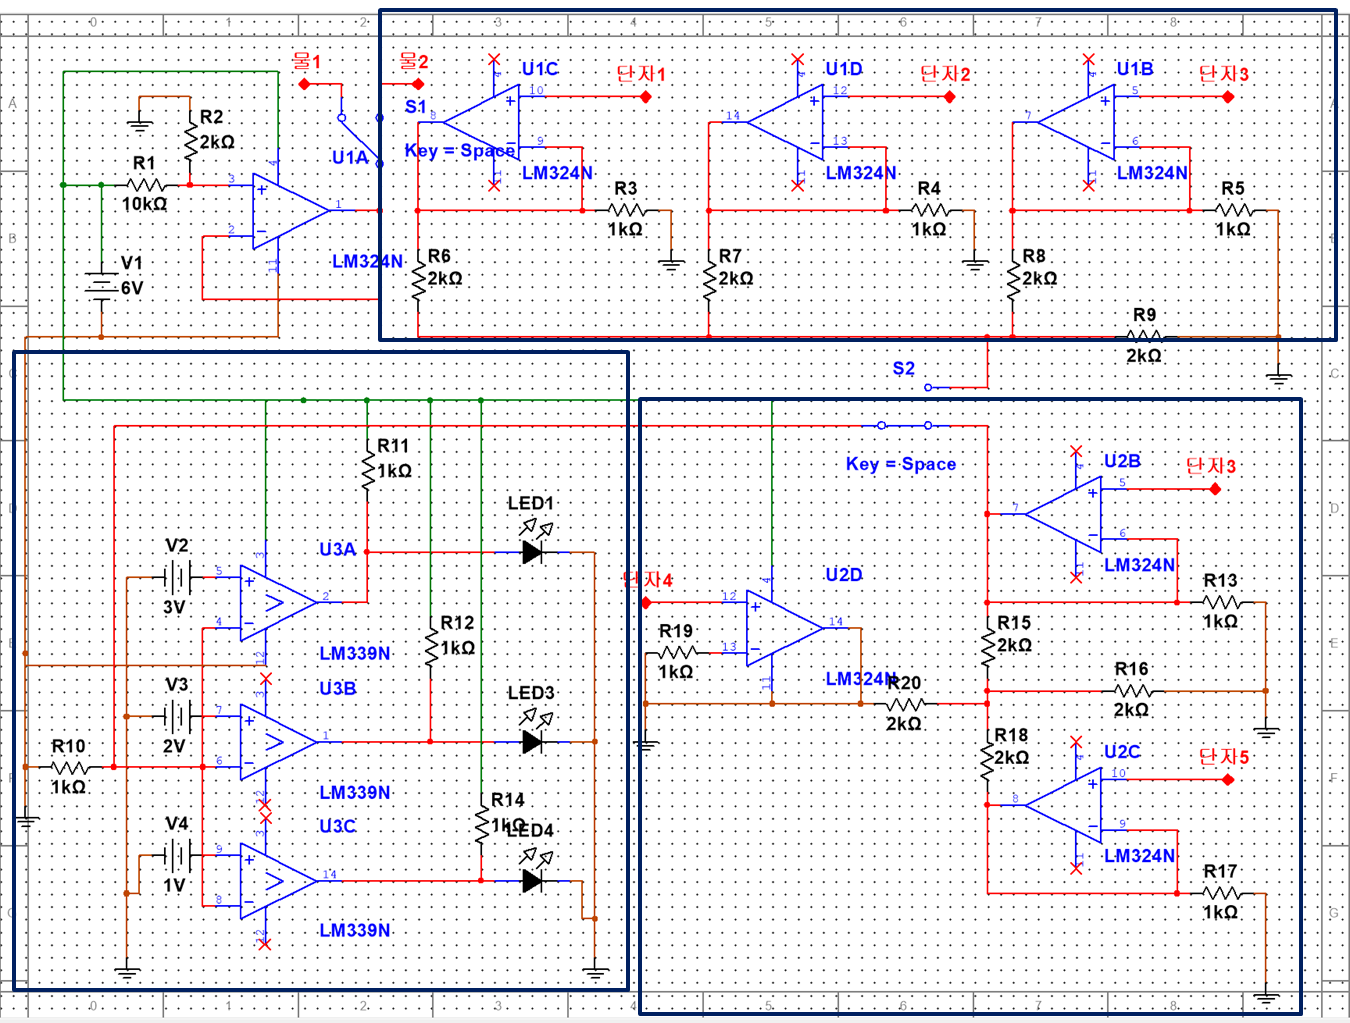
\includegraphics[width=\linewidth]{2nd.png}
  \caption{1차 수정 후의 회로}\label{fig:awesome_image2}
\endminipage\hfill
\minipage{0.32\textwidth}
  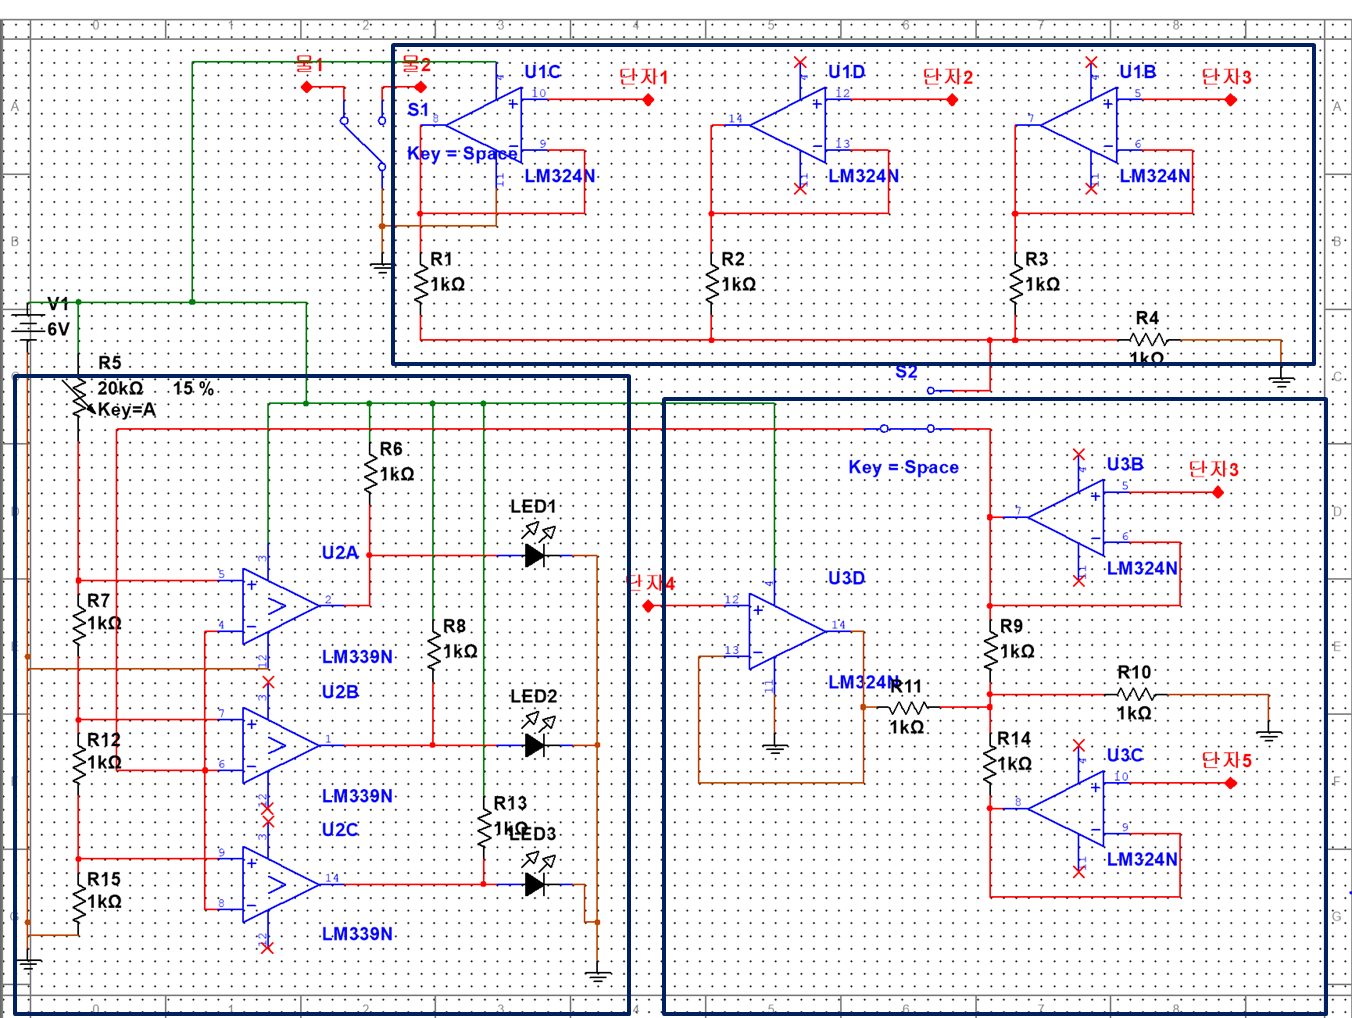
\includegraphics[width=\linewidth]{3rd.png}
  \caption{최종 회로}\label{fig:awesome_image3}
\endminipage
\end{figure}
아두이노 회로에서의 문제점은 물에 접촉하는 전선에 전류가 흐를 수 있었기에 전기분해가 일어날 뿐만이 아니라 물의 저항이 입력에 영향을 준다는 점이었다. 이를 해결하기 위하여 물에 전류가 흐르지 않도록 설계를 하였다. 구체적으로는, 물에 접촉하는 전선이 입력 저항이 큰 단자에 연결되도록 하였다. 가능한 소자들 중에서 가장 입력 저항이 큰 소자는 op amp의 입력 단자였다. 특히 실험실에 있는 LM324N 소자의 입력 저항은 수십 M$\Omega$ 이상으로, 물의 저항인 수십 k$\Omega$에 비교해서 유의미하게 크다는 것을 확인할 수 있다. 이에 컵 안에 노출되는 전선은 입력 저항이 op amp의 입력 저항과 일치하는 non-inverting amplifier의 + 단자에 연결되도록 했다. 이 때 문제점은 전선이 물에 연결되지 않았을 때, 즉 전선이 floating 상태일 때 op amp의 출력이었다. Op amp의 종류에 따라 floating input에 대한 반응이 예측 가능할 수도 있고 랜덤할 수도 있기 때문이다. LM324N의 경우, 입력 단자에 쓰이는 트랜지스터의 특성 상 bias current가 바깥으로 흘러나가기에 입력이 floating이면 positive saturation이 된다. 즉, LM324N은 입력이 물에 접촉할 때와 접촉하지 않을 때가 확실히 구분되는 출력을 내보내는, 이 프로젝트의 목적에 적절한 소자이다.

위와 같은 LM324N의 특성을 파악한 후에는 기능을 추가하고 회로를 경량화하는 일을 반복했다. 각 과정을 설명하면 :
\begin{enumerate}
    \item 중간발표까지의 회로
    \begin{itemize}
        \item \textbf{기능}: 물을 따르는 중에만 잔량을 1/4 간격으로 확인.
        \item \textbf{전선이 물에 접촉되었을 때의 예상 출력}: \underline{물에는} voltage follower로 인가한 1[V]가 주어져 있다. \underline{전선은} GND와 - 단자 사이에 1[k$\Omega$], - 단자와 output 사이에 저항이 없는 non-inverting amp의 + 단자에 연결되어있다. 이 \underline{amp들의 출력들은} 2[k$\Omega$] 저항들로만 입력을 받는 op amp adder를 통해 더해진다. 전선이 물에 연결되지 않았을 때에는 positive saturation인 약 4.7[V](supply voltage 6[V]에서 1.3[V] 아래)가 나오고 연결되었을 때에는 1[V]가 나오기 때문에 3개가 다 연결되지 않았을 때에는 약 4.7 $\times$ 3 $\div$ 4 $\approx$ 3.5[V]가 출력이 되고, 이후에 연결이 하나씩 될 때마다 (4.7 - 1) $\div$ 4 $\approx$ 0.92[V]씩 출력이 떨어진다. 이 떨어지는 구간마다 threshold를 설정하여 comparator를 통해 LED에 전원을 공급한다. Threshold는 6[V]의 supply를 20[k$\Omega$]의 가변저항 한개와 1[k$\Omega$]의 저항으로 divide하여 만들었으며, 가변저항을 쓴 이유는 supply voltage에 따라 threshold를 조절할 수 있게 하기 위해서이다.
        \item Figure 2에서 확인을 하면, 우측 상단의 테두리가 non-inverting amp, 우측 하단의 테두리가 comparator, 좌측의 테두리가 adder, 좌측 상단이 물에 주는 1[V]임을 확인할 수 있다.
    \end{itemize}
    \item 1차 수정 후의 회로
    \begin{itemize}
        \item \textbf{기능}: 용기를 수평으로 놓았을 때의 잔량과 따르는 중의 잔량을 1/4 간격으로 확인.
        \item \textbf{전선이 물에 접촉되었을 때의 예상 출력}: \underline{물에는} voltage follower로 인가한 1[V]가 주어져 있다. \underline{전선은} GND와 - 단자 사이에 1[k$\Omega$], - 단자와 output 사이에 저항이 없는 non-inverting amp의 + 단자에 연결되어있다. 이 \underline{amp들의 출력들은} 2[k$\Omega$] 저항들로만 입력을 받는 adder를 통해 더해진다. 이 adder에는 op amp가 사용되지 않는다. 원래 non-inverting adder의 + 단자에 연결되어야 할 회로가 comparator의 입력에 바로 연결되어있다. 물에 접촉하는 전선의 개수에 따라 출력되는 adder의 전압은 중간 발표 때와 동일하다. Mode 1(따르는 중)과 Mode 2(용기 수평)의 출력과 각 Mode에서 1[V]가 인가되어야 하는 위치(Mode 1에서는 따르는 곳 근처, Mode 2에서는 용기 바닥)는 SPDT 스위치로 조절이 된다.
        \item Figure 3에서, 우측 상단 테두리가 Mode 1의 non-inverting amp와 adder, 우측 하단 테두리가 Mode 2, 좌측 테두리가 comparator, 좌측 상단이 물에 주는 1[V]임을 확인할 수 있다.
        \item \textbf{수정된 사항}: 기능 추가, adder에 쓰이는 op amp 삭제.
    \end{itemize}
    \item 최종 회로
    \begin{itemize}
        \item \textbf{기능}: 용기를 수평으로 놓았을 때의 잔량과 따르는 중의 잔량을 1/4 간격으로 확인.
        \item \textbf{전선이 물에 접촉되었을 때의 예상 출력}: \underline{물에는} GND가 연결되어있다. \underline{전선은} voltage follower의 + 단자에 연결되어있다. 이 \underline{buffer들의 출력들은} 1[k$\Omega$] 저항들로만 입력을 받는 adder를 통해 더해진다. 이 adder에는 op amp가 사용되지 않는다. 물에 접촉하는 전선의 개수에 따라 출력되는 adder의 전압은 약 3.5[V]에서 시작하는 것은 이전과 동일하지만 (4.7 - 0) $\div$ 4 $\approx$ 1.17[V]씩 떨어진다. Mode 1(따르는 중)과 Mode 2(용기 수평)의 출력 중 comparator에 들어가는 것과 각 Mode에서 GND가 연결되어야 하는 위치(Mode 1에서는 따르는 곳 근처, Mode 2에서는 용기 바닥)는 SPDT 스위치로 조절이 된다.
        \item Figure 4에서 확인을 하면, 우측 상단 테두리가 Mode 1의 voltage follower와 adder, 우측 하단 테두리가 Mode 2, 좌측 테두리가 comparator, 좌측 상단이 물에 주는 GND임을 확인할 수 있다.
        \item \textbf{수정된 사항}: non-inverting amp에 쓰이는 저항 삭제, 1[V]를 인가해주는 voltage follower 삭제, 저항 1[k$\Omega$]으로 통일.
    \end{itemize}
\end{enumerate}

\begin{figure}[hb]
\centering
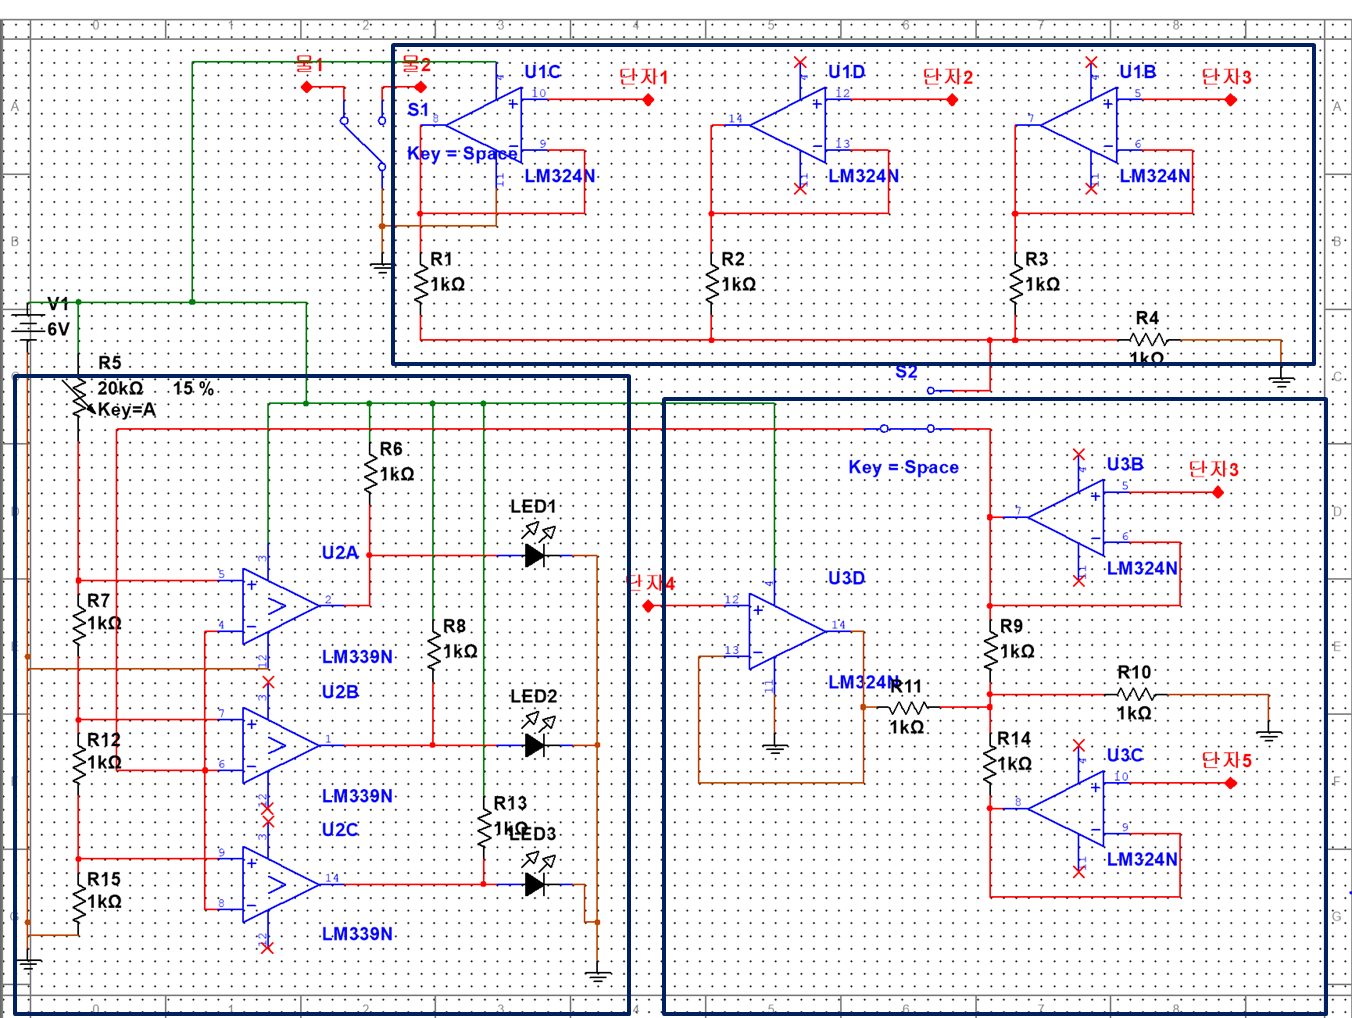
\includegraphics[width=0.5\textwidth]{3rd.png}
\caption{MultiSim으로 시뮬레이션 한 최종 회로}
\end{figure}

위와 같은 과정을 통해, 최종적으로는 quad comparator 하나, quad op amp 2개, 1[k$\Omega$] 저항 14개와 20[k$\Omega$] 가변 저항 하나, 그리고 LED 3개로만 이루어진 효율적인 회로를 구성할 수 있었다.

\subsection{용기 설계}
\begin{figure}[hb]
\centering
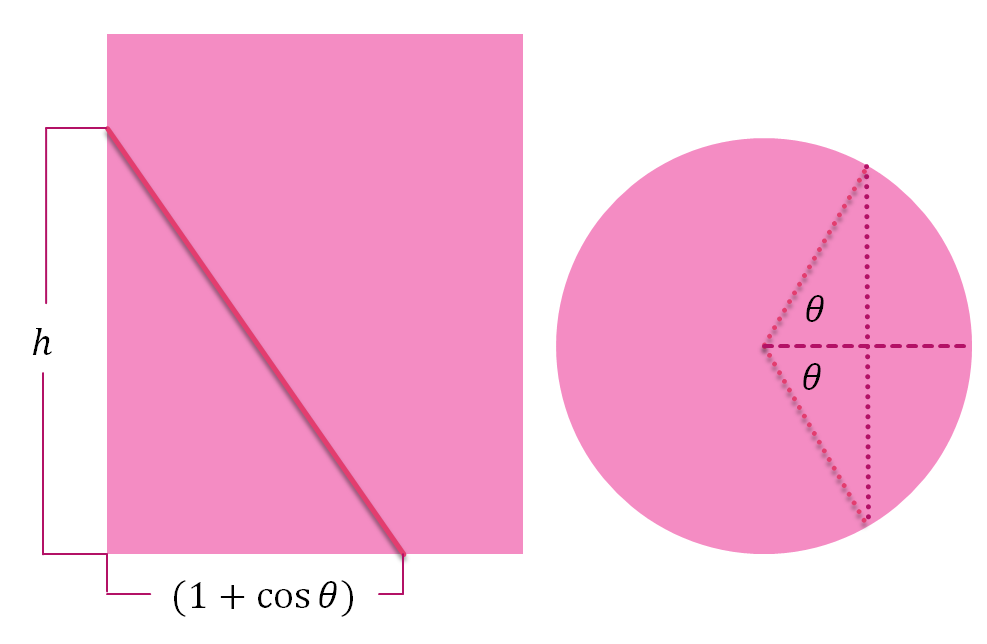
\includegraphics[width=0.5\textwidth]{cup.PNG}
\caption{이상적인 원기둥 용기}
\end{figure}

전선이 물에 연결되면 원하는 출력을 내는 회로를 구성하였으므로, 전선을 용기에 어떻게 배치해야하는지를 설계하는 과정이 필요하다. 이론적인 설계를 하기 위해서 먼저 용기를 완벽한 원기둥이라고 가정했으며, 원기둥을 scaling해서 밑면의 반지름이 1, 높이가 H인 원기둥이라고 가정을 했다. 또한, 수면은 완벽한 평면이고, 수면이 옆면과 높이 h인 지점까지 교점을 가지며, 수면과 밑면의 교선은 Figure 6의 오른쪽 그림과 같이 $1 + \cos{\theta}$ 지점에서 이루어진다고 가정을 했다. 이 때 수면과 밑면 사이의 부피를 구해보면, Figure 6의 오른쪽 그림에서 가로선을 오른쪽으로 향하는 y축, 세로선을 아래로 향하는 x축으로 잡았을 때 $z = -\frac{h}{1+\cos{\theta}}(y-\cos{\theta})$ 평면과 xy 평면 사이를 $r\in[0, 1]$, $\phi\in[\pi/2+\theta, 5\pi/2-\theta]$(극좌표계에서 $\theta$ 대신 $\phi$를 썼다)와 Figure 6의 오른쪽 그림의 이등변삼각형의 합집합에서 적분하면 된다.

이 때 극좌표계로 나타난 부분에서의 적분은:
\begin{equation}
    2\times\int_{-\frac{\pi}{2}}^{\frac{\pi}{2}-\theta}\int_{0}^{1}-\frac{h}{1+\cos{\theta}}(r\sin{\phi}-\cos{\theta})rdrd\phi = 2\times(\frac{h\sin{\theta}}{3(1+\cos{\theta})}+\frac{h\cos{\theta}}{2(1+\cos{\theta})}(\pi-\theta))
\end{equation}
으로 나오며, 이등변삼각형 부분의 적분은:
\begin{equation}
    2\times\int_{0}^{\cos{\theta}}\int_{0}^{\tan{\theta}y}-\frac{h}{1+\cos{\theta}}(y-\cos{\theta})dxdy = \frac{h\sin{\theta}\cos^2{\theta}}{3(1+\cos{\theta})}
\end{equation}
이 나오기에 총 부피는:
\begin{equation}
    V(h, \theta) = \frac{h}{1+\cos{\theta}}(\frac{\sin{\theta}}{3}(\cos^2{\theta}+2)+\cos{\theta}(\pi-\theta))
\end{equation}
가 나온다. 볼 수 있다시피, $h$에 대한 식과 $\theta$에 대한 식으로 완전히 분리된다. 물을 따르고 있는 경우에는 $h=H$이기 때문에, 뒤에 붙어있는 $\theta$에 대한 함수만 고려하면 바닥의 어느 위치에 수면이 놓여있으면 1/4 지점인지를 계산할 수 있다. 이를 그래프로 그려본 것이 Figure 7이다. Figure 7은 조금 더 세밀한 3/8, 2/8, 1/8 지점까지 표시를 해 놓았다.
\begin{figure}[h]
\centering
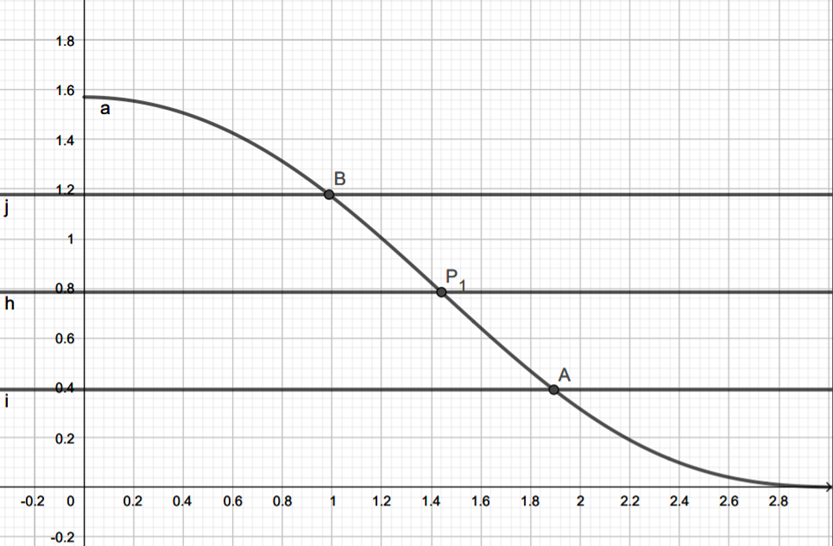
\includegraphics[width=0.3\textwidth]{graph.png}
\caption{원기둥 용기의 경우 관심 지점에서의 $\theta$}
\end{figure}

실제로 용기를 제작할 때에는 인두로도 쉽게 뚫리는 일회용 플라스틱 컵을 사용해서 완벽한 원기둥형은 아니었지만, 최대한 옆면의 기울기가 수직에 가까운 것을 골랐으며, 위 계산 결과와 병행하여 직접 물을 따라보는 실험을 통해 전선을 배치할 지점을 선정했다.
\subsection{실험 결과}
\begin{table}[htb]
\begin{center}
\begin{tabular}{c|c|c|c}
\hline
     Water level & Mode 1 [V] & Mode 2 [V] & Threshold [V]  \\
     \hline
     $1/4$ & 2.5392 & 2.5248 & 3.0102 \\
     $2/4$ & 1.52663 & 1.5250 & 2.0205 \\
     $3/4$ & 0.54449 & 0.48365 & 1.02205 \\
     \hline
\end{tabular}
\end{center}
\caption{PCB로 실험했을 때의 전압의 측정값}
\label{table:1}
\end{table}
이후 회로를 PCB로 제작하여 실제 출력되는 전압을 멀티미터로 측정해봤다. Power Supply로 6.0317[V]를 인가했을 때 출력은 \ref{table:1}과 같이 나온다. 위 표에서 모든 불이 켜졌을 때, 즉 3/4 지점이 넘었을 때 완벽하게 0[V]가 나오지 않는 이유는 전류가 GND를 통해서, 또한 op amp의 bias current에 의해서 물에 들어가기 때문이라고 예상이 된다. 물의 저항이 멀티미터로 쟀을 때 5[cm]정도만 떨어져 있어도 수십 k$\Omega$ 이상으로 컸기 때문에, 10[$\mu$A] 단위 전류도 큰 영향을 끼칠 수 있다. 이러한 문제는 threshold를 조절해서 작동이 잘 되는 지점을 찾으면 해결이 된다.

\section{결론}
지금까지 액체를 용기에서 따라내는 중에, 또 액체를 용기에 따르는 중에 실시간으로 물이 얼마나 남아있는지 알려줄 수 있는 회로를 고안하고 제작을 했다. 결과적으로 완성된 제품은 가격면에서는 general purpose op amp랑 general purpose comparator와 통일된 1[k$\Omega$] 저항을 사용했기에 효율적으로 회로를 구성했다고 할 수 있으며, 기능면에서도 1/4 간격으로는 물의 양을 보여주면서 전기분해가 되는 모습을 확인하지 못했기 때문에 합격이다. 그럼에도 불구하고 이 제품에 남아있는 한계점은 bias current에 의한 전압 변화의 문제 및 컵이 완벽한 원기둥이 아니면서 컵을 완벽하게 기울지 않은 상태와 같은 복잡한 상황에서의 사용이 제한된다는 문제가 있다. 또한, PCB는 용기에 부착하기에 부피가 크고 무게가 나간다는 단점도 있다. 이와 같은 문제점은 voltage follower의 출력에 또 다시 comparator를 달아 완전히 회로를 digital로 바꾸어버리고, 소자를 소형화(surface mount 등)하는 등의 해결책을 통해 해결할 수 있을 것이다. 물론 실제로는 MCU와 같은 소자를 사용하면 해결될 수 있는 문제일지도 모르겠지만, 1/4 간격의 간단한 회로와 같은 경우에는 그보다 훨씬 저렴한 가격으로 같은 성능을 낼 수 있는 가능성이 존재함을 이 프로젝트를 통해 보일 수 있었다.
\begin{thebibliography}{50}

\bibitem{1} Water Level Controls, "Water Level Indicator|What, How, Where, Types, Benefits," \textit{water\\levelcontrols.com,} para. 2, Jun. 1, 2019. [Online]. Available: https://waterlevelcontrols.com\\/water-level-indicator/. [Accessed Jun. 16, 2019].

\end{thebibliography}
\end{document}